\section{Desarrollo de la propuesta}

\subsection{Estrategia experimental}

La etapa experimental se estructuro en cinco experimentos secuenciales: \textit{baseline}, \textit{agregaciones}, \textit{categorizaciones}, \textit{pruning} e \textit{hiperparametros}. Esta nomenclatura coincide con el flujo de experimentacion definido para la sustentacion.

Todas las metricas reportadas en esta seccion se obtienen directamente de los metadatos generados por el pipeline, usando como fuente primaria:

\begin{itemize}
\item \texttt{doc/experiments/tmp\_metrics\_summary.tsv} para metricas consolidadas por experimento y modelo.
\item \texttt{doc/experiments/exp\_05\_hyperparameter\_search/models/<modelo>/plots/plot\_metadata.json} para metricas operativas detalladas del duelo final.
\end{itemize}

\subsection{Experimento 1: Baseline}

En el experimento baseline se evaluaron siete algoritmos con configuracion base para establecer la linea de referencia.

\begin{table}[H]
\centering
\caption{Top 3 modelos por AUC-ROC en el Experimento 1}
\label{tab:exp1-top3}
\begin{tabular}{|l|c|}
\hline
\textbf{Modelo} & \textbf{AUC-ROC} \\ \hline
catboost & 0.6153 \\ \hline
logistic\_regression\_lasso & 0.6055 \\ \hline
xgboost & 0.5950 \\ \hline
\end{tabular}
\end{table}

\begin{figure}[H]
\centering
\begin{subfigure}[b]{0.48\textwidth}
\centering

\includegraphics[width=\textwidth]{../experiments/exp_01_base_models/comparison_plots/roc_comparison.png}
\caption{Comparacion ROC global}
\label{fig:exp1-roc}
\end{subfigure}
\hfill
\begin{subfigure}[b]{0.48\textwidth}
\centering
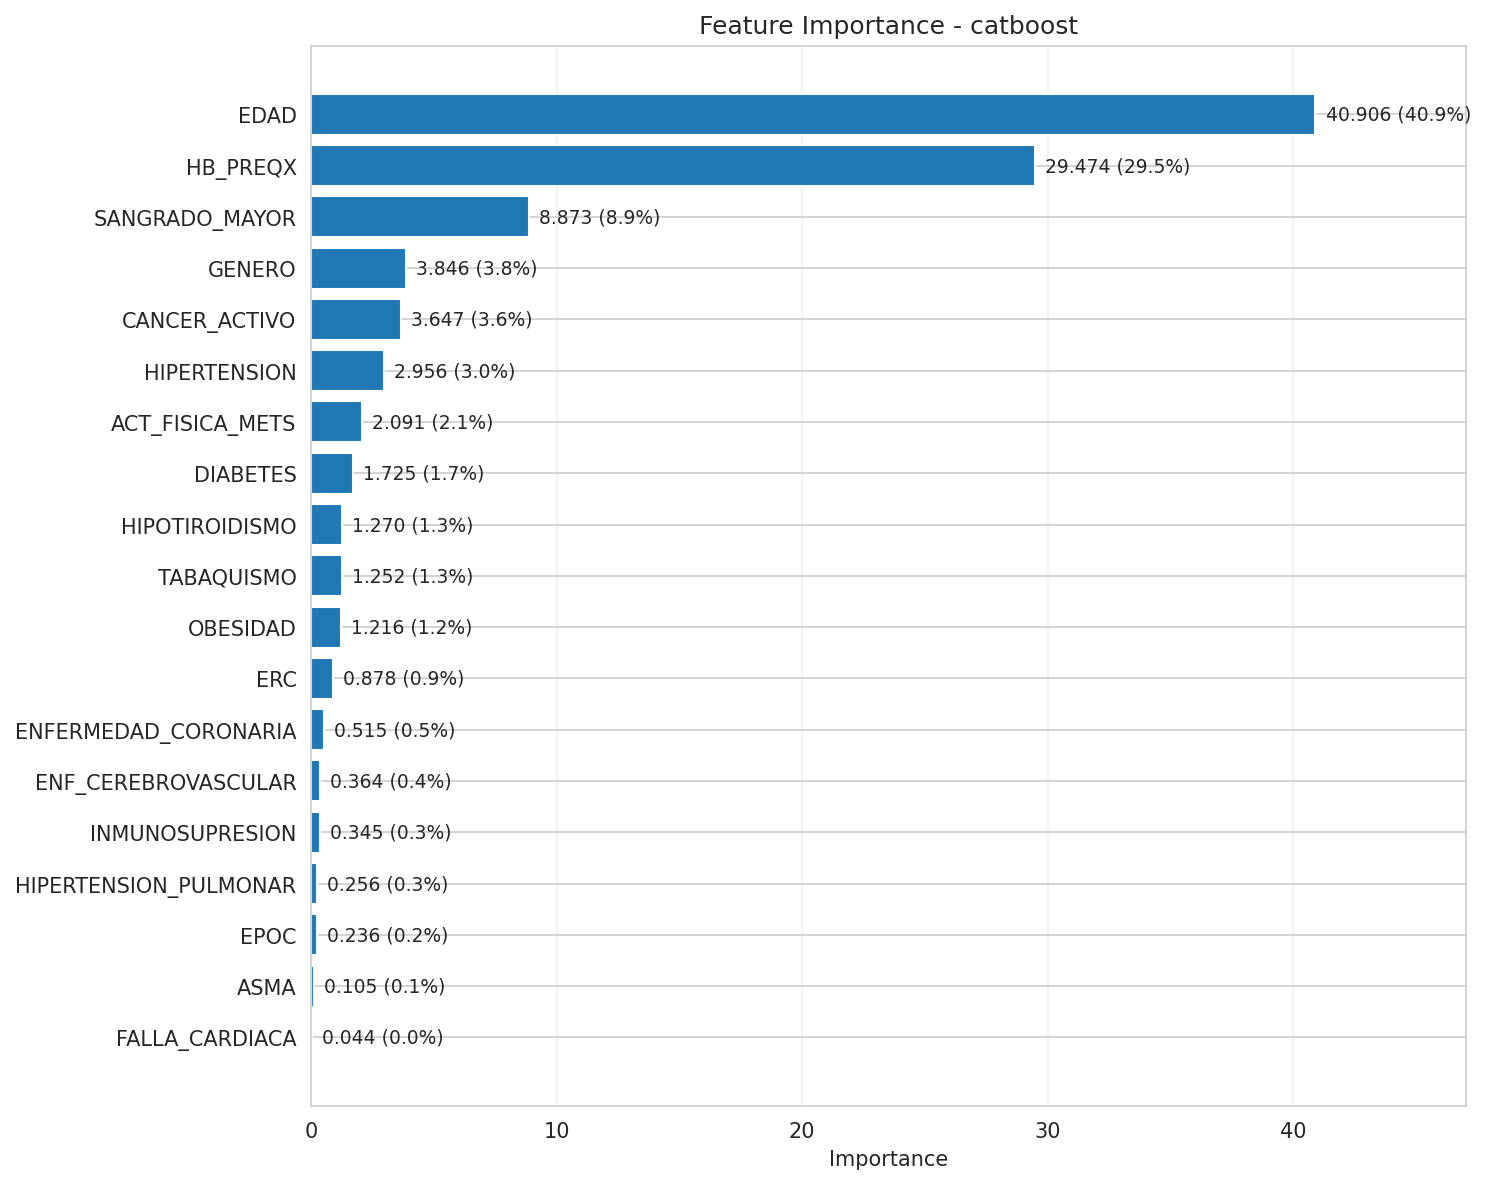
\includegraphics[width=\textwidth]{../experiments/exp_01_base_models/models/catboost/plots/feature_importance.png}
\caption{Importancia variables (catboost)}
\label{fig:exp1-fi-catboost}
\end{subfigure}
\caption{Resultados Experimento 1}
\label{fig:exp1-results}
\end{figure}

\subsection{Experimento 2: Agregaciones}

Se incorporaron variables derivadas y agregaciones clinicas para aumentar la capacidad discriminativa del modelo. El mejor resultado de esta fase fue catboost con AUC-ROC de 0.6192.

\begin{table}[H]
\centering
\caption{Top 3 modelos por AUC-ROC en el Experimento 2}
\label{tab:exp2-top3}
\begin{tabular}{|l|c|}
\hline
\textbf{Modelo} & \textbf{AUC-ROC} \\ \hline
catboost & 0.6192 \\ \hline
logistic\_regression\_lasso & 0.6055 \\ \hline
xgboost & 0.6045 \\ \hline
\end{tabular}
\end{table}

\begin{figure}[H]
\centering
\begin{subfigure}[b]{0.48\textwidth}
\centering

\includegraphics[width=\textwidth]{../experiments/exp_02_aggregated_features/comparison_plots/roc_comparison.png}
\caption{Comparacion ROC global}
\label{fig:exp2-roc}
\end{subfigure}
\hfill
\begin{subfigure}[b]{0.48\textwidth}
\centering

\includegraphics[width=\textwidth]{../experiments/exp_02_aggregated_features/models/catboost/plots/feature_importance.png}
\caption{Importancia variables (catboost)}
\label{fig:exp2-fi-catboost}
\end{subfigure}
\caption{Resultados Experimento 2}
\label{fig:exp2-results}
\end{figure}

\subsection{Experimento 3: Categorizaciones}

Se evaluo la categorizacion de variables continuas en rangos clinicos. El resultado mostro una caida frente al experimento anterior, con mejor AUC-ROC de 0.6134 (catboost), lo cual sugiere perdida de informacion discriminativa al discretizar.

\begin{table}[H]
\centering
\caption{Top 3 modelos por AUC-ROC en el Experimento 3}
\label{tab:exp3-top3}
\begin{tabular}{|l|c|}
\hline
\textbf{Modelo} & \textbf{AUC-ROC} \\ \hline
catboost & 0.6134 \\ \hline
logistic\_regression\_lasso & 0.6037 \\ \hline
xgboost & 0.5950 \\ \hline
\end{tabular}
\end{table}

\begin{figure}[H]
\centering

\includegraphics[width=0.85\textwidth]{../experiments/exp_03_categorical_features/comparison_plots/roc_comparison.png}
\caption{Comparacion ROC global del Experimento 3}
\label{fig:exp3-roc}
\end{figure}

% \begin{figure}[H]
% \centering
% 
\includegraphics[width=0.78\textwidth]{../experiments/exp_03_categorical_features/models/catboost/plots/feature_importance.png}
% \caption{Importancia de variables del modelo lider (catboost) en el Experimento 3}
% \label{fig:exp3-fi-catboost}
% \end{figure}
% Nota: Grafica de importancia de variables omitida debido a archivo corrupto

\subsection{Experimento 4: Pruning}

La cuarta fase se enfoco en reducir ruido y mantener solo caracteristicas con mayor utilidad predictiva. Se descartaron siete variables de baja ocurrencia (criterio minimo: 10 casos) que mostraron aporte marginal al desempeno discriminativo en fases previas.

\begin{table}[H]
\centering
\caption{Variables descartadas en feature pruning}
\label{tab:exp4-pruned-vars}
\begin{tabular}{|l|}
\hline
\textbf{Variable} \\ \hline
ENFERMEDAD\_CORONARIA \\ \hline
FALLA\_CARDIACA \\ \hline
INMUNOSUPRESION \\ \hline
HIPERTENSION\_PULMONAR \\ \hline
EPOC \\ \hline
ASMA \\ \hline
ENF\_CEREBROVASCULAR \\ \hline
\end{tabular}
\end{table}

Tras la eliminacion de estas variables, catboost volvio a liderar con AUC-ROC de 0.6237, manteniendo resultados competitivos con un conjunto de caracteristicas mas compacto.

\begin{table}[H]
\centering
\caption{Top 4 modelos por AUC-ROC en el Experimento 4}
\label{tab:exp4-top4}
\begin{tabular}{|l|c|}
\hline
\textbf{Modelo} & \textbf{AUC-ROC} \\ \hline
catboost & 0.6237 \\ \hline
logistic\_regression\_lasso & 0.6067 \\ \hline
xgboost & 0.6038 \\ \hline
lightgbm & 0.5995 \\ \hline
\end{tabular}
\end{table}

\begin{figure}[H]
\centering
\begin{subfigure}[b]{0.48\textwidth}
\centering

\includegraphics[width=\textwidth]{../experiments/exp_04_feature_pruning/comparison_plots/roc_comparison.png}
\caption{Comparacion ROC global}
\label{fig:exp4-roc}
\end{subfigure}
\hfill
\begin{subfigure}[b]{0.48\textwidth}
\centering

\includegraphics[width=\textwidth]{../experiments/exp_04_feature_pruning/models/catboost/plots/roc_curve_cv.png}
\caption{ROC CV catboost (lider)}
\label{fig:exp4-catboost-roc}
\end{subfigure}
\caption{Resultados Experimento 4}
\label{fig:exp4-results}
\end{figure}

\subsubsection{Comparativa complementaria en pruning}

Para reproducir el analisis de la presentacion, se incorpora la comparativa visual de curvas ROC en CV para los contendientes logistic\_regression\_lasso y xgboost bajo el mismo esquema de poda.

\begin{figure}[H]
\centering
\begin{subfigure}[b]{0.48\textwidth}
\centering

\includegraphics[width=\textwidth]{../experiments/exp_04_feature_pruning/models/logistic_regression_lasso/plots/roc_curve_cv.png}
\caption{Logistic Regression Lasso}
\label{fig:exp4-lasso-roc}
\end{subfigure}
\hfill
\begin{subfigure}[b]{0.48\textwidth}
\centering

\includegraphics[width=\textwidth]{../experiments/exp_04_feature_pruning/models/xgboost/plots/roc_curve_cv.png}
\caption{XGBoost}
\label{fig:exp4-xgb-roc}
\end{subfigure}
\caption{Curvas ROC en CV - Comparativa complementaria Experimento 4}
\label{fig:exp4-roc-comp}
\end{figure}

\subsection{Experimento 5: Hiperparametros}

La fase final realizo optimizacion de hiperparametros para todos los modelos y consolido la comparacion final de desempeno.

\begin{table}[H]
\centering
\caption{Ranking de modelos por AUC-ROC en el Experimento 5}
\label{tab:exp5-ranking}
\begin{tabular}{|c|l|c|}
\hline
\textbf{Ranking} & \textbf{Modelo} & \textbf{AUC-ROC} \\ \hline
1 & random\_forest & 0.6404 \\ \hline
2 & lightgbm & 0.6384 \\ \hline
3 & xgboost & 0.6371 \\ \hline
4 & decision\_tree & 0.6354 \\ \hline
5 & catboost & 0.6215 \\ \hline
6 & logistic\_regression\_lasso & 0.6068 \\ \hline
7 & naive\_bayes & 0.5707 \\ \hline
\end{tabular}
\end{table}

\begin{figure}[H]
\centering
\begin{subfigure}[b]{0.48\textwidth}
\centering

\includegraphics[width=\textwidth]{../experiments/exp_05_hyperparameter_search/comparison_plots/roc_comparison.png}
\caption{Comparacion ROC global}
\label{fig:exp5-roc}
\end{subfigure}
\hfill
\begin{subfigure}[b]{0.48\textwidth}
\centering

\includegraphics[width=\textwidth]{../experiments/exp_05_hyperparameter_search/comparison_plots/roc_boxplot_comparison.png}
\caption{Distribucion AUC-ROC CV}
\label{fig:exp5-roc-boxplot}
\end{subfigure}
\caption{Desempeno comparativo Experimento 5}
\label{fig:exp5-performance}
\end{figure}

\begin{figure}[H]
\centering

\includegraphics[width=0.78\textwidth]{../experiments/exp_05_hyperparameter_search/models/random_forest/plots/feature_importance.png}
\caption{Importancia de variables del modelo lider (random\_forest) en el Experimento 5}
\label{fig:exp5-rf-fi}
\end{figure}

\subsubsection{Comparativa final: Random Forest vs Decision Tree}

Para la decision final se contrasto el mejor modelo discriminativo (random\_forest) frente al mejor candidato interpretable (decision\_tree), usando las metricas de operacion reportadas en \texttt{plot\_metadata.json}.

\begin{table}[H]
\centering
\caption{Comparativa de metricas operativas en el Experimento 5}
\label{tab:exp5-duelo}
\begin{tabular}{|l|c|c|}
\hline
\textbf{Metrica} & \textbf{random\_forest} & \textbf{decision\_tree} \\ \hline
AUC-ROC (CV) & 0.6404 & 0.6354 \\ \hline
Threshold optimo & 0.38 & 0.22 \\ \hline
Recall & 0.8196 & 0.8568 \\ \hline
Specificity & 0.3567 & 0.3154 \\ \hline
Precision & 0.3755 & 0.3713 \\ \hline
NPV & 0.8074 & 0.8235 \\ \hline
F1-score & 0.5150 & 0.5180 \\ \hline
F2-score & 0.6628 & 0.6791 \\ \hline
Accuracy & 0.5051 & 0.4889 \\ \hline
Kappa & 0.1344 & 0.1280 \\ \hline
\end{tabular}
\end{table}

Desde el criterio clinico de deteccion temprana, random\_forest se prioriza por mayor AUC-ROC y mejor balance recall-especificidad. En paralelo, decision\_tree conserva valor practico por su transparencia estructural y mayor interpretabilidad para discusion con equipo medico.

\begin{figure}[H]
\centering
\begin{subfigure}[b]{0.48\textwidth}
\centering

\includegraphics[width=\textwidth]{../experiments/exp_05_hyperparameter_search/models/random_forest/plots/roc_curve_cv.png}
\caption{Random Forest (AUC=0.6404)}
\label{fig:exp5-rf-roc}
\end{subfigure}
\hfill
\begin{subfigure}[b]{0.48\textwidth}
\centering

\includegraphics[width=\textwidth]{../experiments/exp_05_hyperparameter_search/models/decision_tree/plots/roc_curve_cv.png}
\caption{Decision Tree (AUC=0.6354)}
\label{fig:exp5-tree-roc}
\end{subfigure}
\caption{Curvas ROC en CV - Experimento 5}
\label{fig:exp5-roc-comp}
\end{figure}

\subsubsection{Estructura e interpretacion del arbol de decision}

El modelo \texttt{decision\_tree} optimizado genera un clasificador binario con profundidad maxima de 7 niveles y 27 hojas terminales. La figura \ref{fig:exp5-tree-structure} presenta la estructura completa del arbol.

\begin{figure}[H]
\centering

\includegraphics[width=0.98\textwidth]{../experiments/exp_05_hyperparameter_search/models/decision_tree/plots/decision_tree_full.png}
\caption{Estructura completa del arbol de decision optimizado (Experimento 5)}
\label{fig:exp5-tree-structure}
\end{figure}

\textbf{Analisis de la estructura de decision:}

\begin{itemize}
\item \textbf{Configuracion general:} Clasificador binario basado en criterio de Gini. La Clase 0.0 (naranja, shock ausente) representa el 67.9\% de casos en el nodo raiz. La Clase 1.0 (azul, shock presente) se concentra en ramas especificas de la derecha del arbol.

\item \textbf{Variables con mayor poder discriminativo:} \texttt{SANGRADO\_MAYOR} actua como variable de division en el nodo raiz (critica para identificacion temprana). \texttt{EDAD} modula la probabilidad de shock en ambas ramas principales. \texttt{HB\_PREQX} y \texttt{SINDROME\_METABOLICO} refinan la clasificacion en nodos internos.

\item \textbf{Logica de decision principal:} La rama de \texttt{SANGRADO\_MAYOR} $> 1.582$ constituye la ruta critica para identificar casos de shock (Clase 1.0), especialmente cuando se combina con \texttt{EDAD} $> 0.236$ (Z-score estandarizado), generando alta pureza de clase positiva. Si el sangrado es $\leq 1.582$, la probabilidad de shock es minima ($<$ 0.20), salvo interacciones especificas entre edad y hemoglobina preoperatoria.

\item \textbf{Perfil de riesgo maximo:} El riesgo mas alto de shock (Clase 1.0) se concentra en pacientes con valores altos de sangrado intraoperatorio (Z-score $> 1.582$) y edades especificas: mayores de 65 anos (Z-score $> 0.236$) o en rango medio de 50-65 anos (Z-score entre $-0.877$ y $0.236$). La combinacion de estas condiciones eleva la probabilidad de shock por encima del 60\% en hojas terminales especificas.
\end{itemize}

\subsubsection{Comparativas visuales del duelo final}

Adicionalmente se incluyen las mismas comparativas visuales presentadas en sustentacion para contrastar estabilidad y comportamiento operativo entre random\_forest y decision\_tree.

\begin{figure}[H]
\centering
\begin{subfigure}[b]{0.48\textwidth}
\centering

\includegraphics[width=\textwidth]{../experiments/exp_05_hyperparameter_search/models/random_forest/plots/cv_fold_plots/cv_fold_roc_auc.png}
\caption{Random Forest}
\label{fig:exp5-rf-cv-box}
\end{subfigure}
\hfill
\begin{subfigure}[b]{0.48\textwidth}
\centering

\includegraphics[width=\textwidth]{../experiments/exp_05_hyperparameter_search/models/decision_tree/plots/cv_fold_plots/cv_fold_roc_auc.png}
\caption{Decision Tree}
\label{fig:exp5-tree-cv-box}
\end{subfigure}
\caption{Boxplot de AUC-ROC por fold en CV - Experimento 5}
\label{fig:exp5-cv-boxplot-comp}
\end{figure}

\begin{figure}[H]
\centering
\begin{subfigure}[b]{0.48\textwidth}
\centering

\includegraphics[width=\textwidth]{../experiments/exp_05_hyperparameter_search/models/random_forest/plots/perf_precision_npv.png}
\caption{Random Forest}
\label{fig:exp5-rf-precision-npv}
\end{subfigure}
\hfill
\begin{subfigure}[b]{0.48\textwidth}
\centering

\includegraphics[width=\textwidth]{../experiments/exp_05_hyperparameter_search/models/decision_tree/plots/perf_precision_npv.png}
\caption{Decision Tree}
\label{fig:exp5-tree-precision-npv}
\end{subfigure}
\caption{Comparativa Precision-NPV - Experimento 5}
\label{fig:exp5-precision-npv-comp}
\end{figure}

\begin{figure}[H]
\centering
\begin{subfigure}[b]{0.48\textwidth}
\centering

\includegraphics[width=\textwidth]{../experiments/exp_05_hyperparameter_search/models/random_forest/plots/perf_f1_f2.png}
\caption{Random Forest}
\label{fig:exp5-rf-f1-f2}
\end{subfigure}
\hfill
\begin{subfigure}[b]{0.48\textwidth}
\centering

\includegraphics[width=\textwidth]{../experiments/exp_05_hyperparameter_search/models/decision_tree/plots/perf_f1_f2.png}
\caption{Decision Tree}
\label{fig:exp5-tree-f1-f2}
\end{subfigure}
\caption{Comparativa F1-F2 - Experimento 5}
\label{fig:exp5-f1-f2-comp}
\end{figure}

\begin{figure}[H]
\centering
\begin{subfigure}[b]{0.48\textwidth}
\centering

\includegraphics[width=\textwidth]{../experiments/exp_05_hyperparameter_search/models/random_forest/plots/kappa.png}
\caption{Random Forest}
\label{fig:exp5-rf-kappa}
\end{subfigure}
\hfill
\begin{subfigure}[b]{0.48\textwidth}
\centering

\includegraphics[width=\textwidth]{../experiments/exp_05_hyperparameter_search/models/decision_tree/plots/kappa.png}
\caption{Decision Tree}
\label{fig:exp5-tree-kappa}
\end{subfigure}
\caption{Comparativa Kappa - Experimento 5}
\label{fig:exp5-kappa-comp}
\end{figure}

\begin{figure}[H]
\centering
\begin{subfigure}[b]{0.48\textwidth}
\centering

\includegraphics[width=\textwidth]{../experiments/exp_05_hyperparameter_search/models/random_forest/plots/confusion_matrix_normalized.png}
\caption{Random Forest}
\label{fig:exp5-rf-confusion}
\end{subfigure}
\hfill
\begin{subfigure}[b]{0.48\textwidth}
\centering

\includegraphics[width=\textwidth]{../experiments/exp_05_hyperparameter_search/models/decision_tree/plots/confusion_matrix_normalized.png}
\caption{Decision Tree}
\label{fig:exp5-tree-confusion}
\end{subfigure}
\caption{Matriz de confusion normalizada - Experimento 5}
\label{fig:exp5-confusion-comp}
\end{figure}

\subsection{Evolucion global y cierre de fase experimental}

\begin{table}[H]
\centering
\caption{Evolucion del mejor AUC-ROC por experimento}
\label{tab:evolucion-auc}
\begin{tabular}{|l|c|c|}
\hline
\textbf{Experimento} & \textbf{Mejor modelo} & \textbf{AUC-ROC} \\ \hline
Exp 1 (Baseline) & catboost & 0.6153 \\ \hline
Exp 2 (Features agregadas) & catboost & 0.6192 \\ \hline
Exp 3 (Variables categoricas) & catboost & 0.6134 \\ \hline
Exp 4 (Feature pruning) & catboost & 0.6237 \\ \hline
Exp 5 (Hyperparameter search) & random\_forest & 0.6404 \\ \hline
\end{tabular}
\end{table}

En terminos absolutos, la mejora del mejor modelo entre el inicio y el cierre experimental fue:

$$\Delta AUC = 0.6404 - 0.6153 = 0.0251$$

Adicionalmente, el modelo interpretable \texttt{decision\_tree} paso de AUC=0.5557 en Exp 1 a AUC=0.6354 en Exp 5, con una mejora absoluta de 0.0797.
